\documentclass{beamer}
\usepackage[utf8]{inputenc}

%\usepackage{utopia} %font utopia imported

\usetheme{Berkeley}
\usecolortheme{default}

%------------------------------------------------------------
%This block of code defines the information to appear in the
%Title page
\title[Analytical Workflows] %optional
{Analytical Workflows}

\subtitle{IB 516}

\author[] % (optional)
{Developed by Mark Novak and Ben Dalziel}

\institute[OSU] % (optional)
{
  \inst{}%
  Dept. of Integrative Biology\\
  Oregon State University
%  \and
%  \inst{2}%
%  Faculty of Chemistry\\
%  Very Famous University
}

\date[Fall2021] % (optional)
{}

%\logo{\includegraphics[height=1.5cm]{lion-logo.jpg}}

%End of title page configuration block
%------------------------------------------------------------



%------------------------------------------------------------
%The next block of commands puts the table of contents at the
%beginning of each section and highlights the current section:

\AtBeginSection[]
{
  \begin{frame}
    \frametitle{Overview}
    \tableofcontents[currentsection]
  \end{frame}
}

%------------------------------------------------------------

\hypersetup{pdfpagemode=FullScreen} % This will auto-start the pdf presentation in fullscreen mode

%------------------------------------------------------------

\begin{document}

%The next statement creates the title page.
\frame{\titlepage}

%---------------------------------------------------------
%This block of code is for the table of contents after
%the title page
\begin{frame}
    \frametitle{Overview}
    \tableofcontents
\end{frame}

%---------------------------------------------------------

\section{Philosophy}

%---------------------------------------------------------

\begin{frame}{Course Principles}

    \frametitle{Course Principles}

        \begin{block}{Automation}
            Doing science involves repetition at multiple levels.\\Automation is more efficient and reduces mistakes.
        \end{block}

        \begin{block}{Reproducibility}
            Science should be reproducible, by others and you.\\Your work must be \emph{readable}, \emph{organized}, and \emph{self-contained}.
        \end{block}

        \begin{block}{Correctness}
            Science's limitations are human. \\We must work in ways that protect against 'bugs'.
        \end{block}

        \footnotetext[1]{ See Allesina \& Wilmes 2019}

\end{frame}

\begin{frame}

    \frametitle{Course Principles}

        \begin{block}{Simplicity}
            Analyses should be coded as simply as possible.\\Clever and readable are often at odds.
        \end{block}

        \begin{block}{Openness}
            Science is a worldwide endeavor.\\It, and access to it, should be free and equitable.
        \end{block}

        \begin{block}{Science as Software Development}
            Science is a $process$ - no final product, just versions and updates.\\Software developers have tools to help.
        \end{block}

        \footnotetext[1]{ See Allesina \& Wilmes 2019}

\end{frame}

%---------------------------------------------------------
\section{Course Outline}

%---------------------------------------------------------

\subsection{Website \& Schedule}

\begin{frame}
    \frametitle{Website \& Schedule}
    \url{https://github.com/analyticalworkflows}

\end{frame}

%---------------------------------------------------------

\subsection{Syllabus}
% On website

%---------------------------------------------------------

\subsection{Accountabilibuddies}

\begin{frame}
  \frametitle{Accountabilibuddies}

  \begin{itemize}
    \item Weekly check-in
    \begin{itemize}
      \item[] \emph{- goals/deadlines, accomplishments, sticking-points}
      \item[] \emph{- final 10 min. of Thursday class}
    \end{itemize}
    \item Randomized pairing
    \begin{itemize}
     % \item[] \emph{- via automated Zoom breakout rooms right now}
      \item[] \emph{- re-randomized week 6}
    \end{itemize}
  \end{itemize}

\end{frame}

%---------------------------------------------------------

\section{Accounts \& Apps}

%---------------------------------------------------------
%\subsection{Zoom vs. Discord}

%\begin{frame}
 %   \frametitle{To Zoom or not to Zoom?}
 %  \url{https://discord.com}
  %  \begin{figure}
    %    \centering
      %  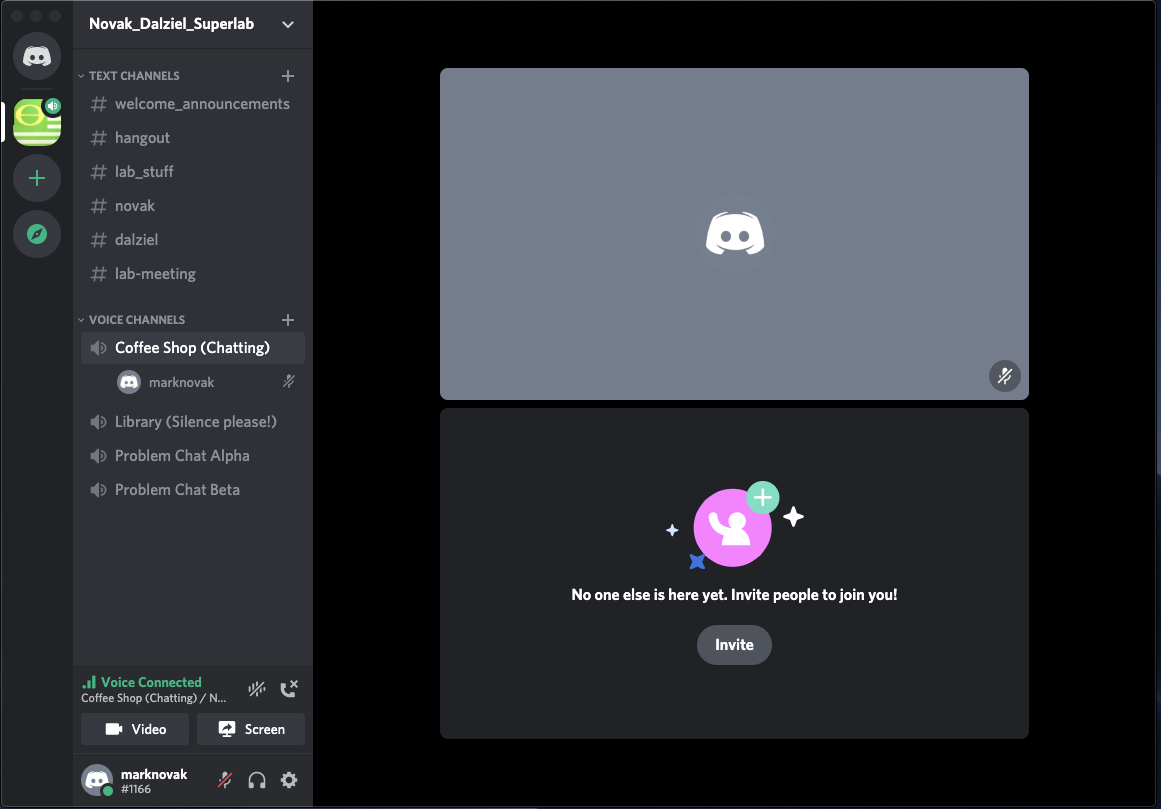
\includegraphics[width = 1\textwidth]{figs/Discord.png}
%  \end{figure}

%\end{frame}

%---------------------------------------------------------
\subsection{Required}

\begin{frame}
    \frametitle{What you'll need}

\begin{columns}

\column{0.5\textwidth}

Software
    \begin{itemize}
        \item \texttt{Git}
        \item \LaTeX
    \end{itemize}
Accounts
    \begin{itemize}
        \item GitHub\footnotemark
    \end{itemize}

\LaTeX{} editor
    \begin{itemize}
        \item Stand-alone {\tiny \emph{(TeXstudio, Atom,...)} \par}
        \item Online {\tiny \emph{(OverLeaf,...)} \par}
    \end{itemize}
\texttt{Git} GUI 
    \begin{itemize}
        \item Sourcetree
        \item GitHub Desktop
    \end{itemize}

\column{0.5\textwidth}
   \begin{figure}
    \centering
    
\includegraphics[width = 0.9\textwidth]{figs/phd101212s.png}
  \end{figure}
\end{columns}
\footnotetext[1]{Please send me your username.}
\end{frame}

%---------------------------------------------------------

\section{Project Proposals}

%---------------------------------------------------------

\begin{frame}
    \frametitle{Project Proposals}

    \begin{block}{Primary Goal}
        To develop more effective research skills.
    \end{block}

    \begin{block}{Secondary Goal}
        To make significant progress on your thesis.
    \end{block}

    \begin{block}{Our belief}
        We can achieve both in this course!
    \end{block}

Let's get started!\\
        \href{https://github.com/analyticalworkflows/TeachingMaterials/tree/master/classes/ProjectProposal}{.../TeachingMaterials/classes/ProjectProposal}


\end{frame}

%---------------------------------------------------------

\section{Our hope}

%---------------------------------------------------------

\begin{frame}
    \frametitle{We're all learning...}

    %This is my first ever ``remote'' course.\\
    %This is my first ever \LaTeX{} Beamer presentation!

    %\bigskip

    \begin{itemize}
        \item Be kind to yourself
        \item Support each other
    \end{itemize}

	\bigskip

    %\begin{block}{Integrity}
    %  Doing the right thing, even when no one is watching.
    %\end{block}

\end{frame}
%---------------------------------------------------------


\end{document}
